\subsubsection{Synchronization and Communication Ordering in \openshmem}

\rcomment{Pasha: Since this section includes barrier, it is relevant for all the rest of the one sided operations. I would consider to move it to a standalone section with all the relevant calls.}
In the presence of the \openshmem's one-sided communication, synchronization and ordering becomes critical. The updates via \FUNC{shmem\_puts} cannot be guaranteed until some form of synchronization or ordering is introduced by the application programmer. The table below gives the different synchronization and ordering options and situations where they may be useful.\\

\begin{tabular}{p{0.2\textwidth} | p{0.7\textwidth}}
\hline 
\textbf{\openshmem  \ac{API}} & \centering \textbf{Working of \openshmem \ac{API}} \tabularnewline
\hline 
\hline 
{Point-to-point synchronization}\\
\FUNC{shmem\_wait}, \FUNC{shmem\_wait\_until} 
&
\raisebox{-\totalheight}{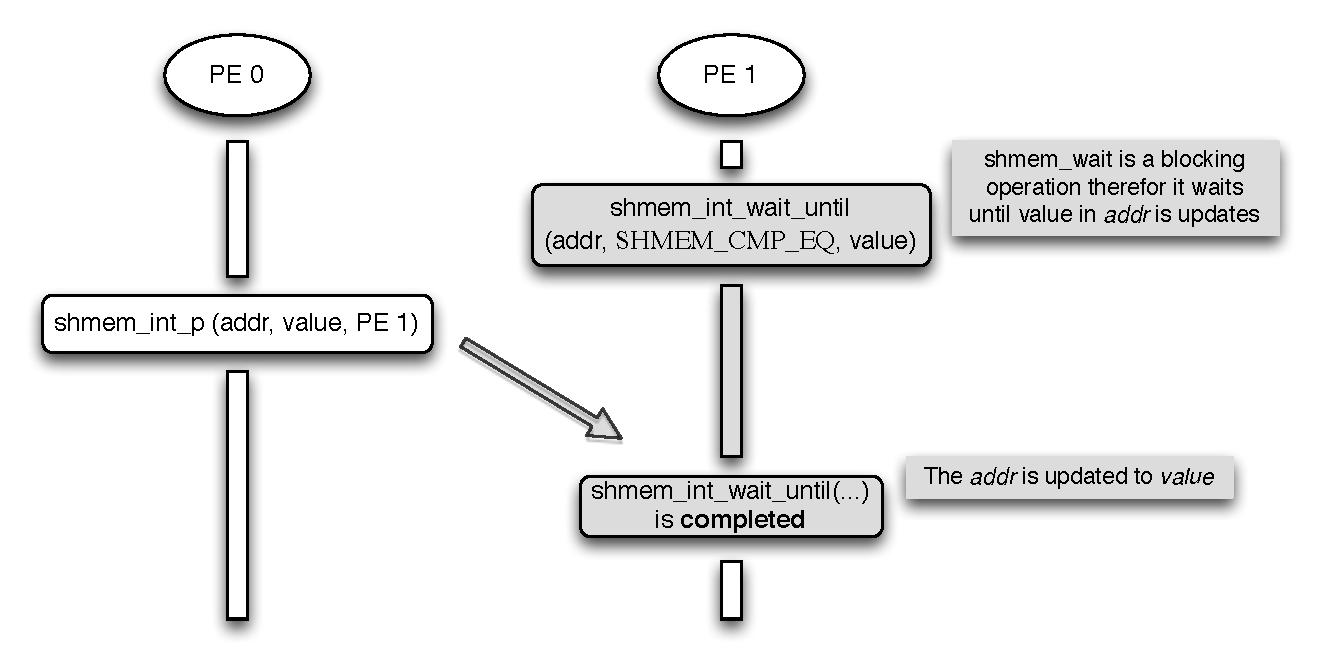
\includegraphics[width=0.7\textwidth]{diagrams/updated/wait}}
\end{tabular}

\begin{tabular}{p{0.2\textwidth} | p{0.7\textwidth}}
{}
&
{ Waits for a symmetric variable to be updated by a remote \ac{PE}. Should be used when computation on the local \ac{PE} cannot proceed without the value that the remote \ac{PE} is to update.} \tabularnewline
\hline 
\end{tabular}

\begin{tabular}{p{0.2\textwidth} | p{0.7\textwidth}}
Ordering puts issued by a local \ac{PE} \\
\FUNC{shmem\_fence} 
& 
\raisebox{-\totalheight}{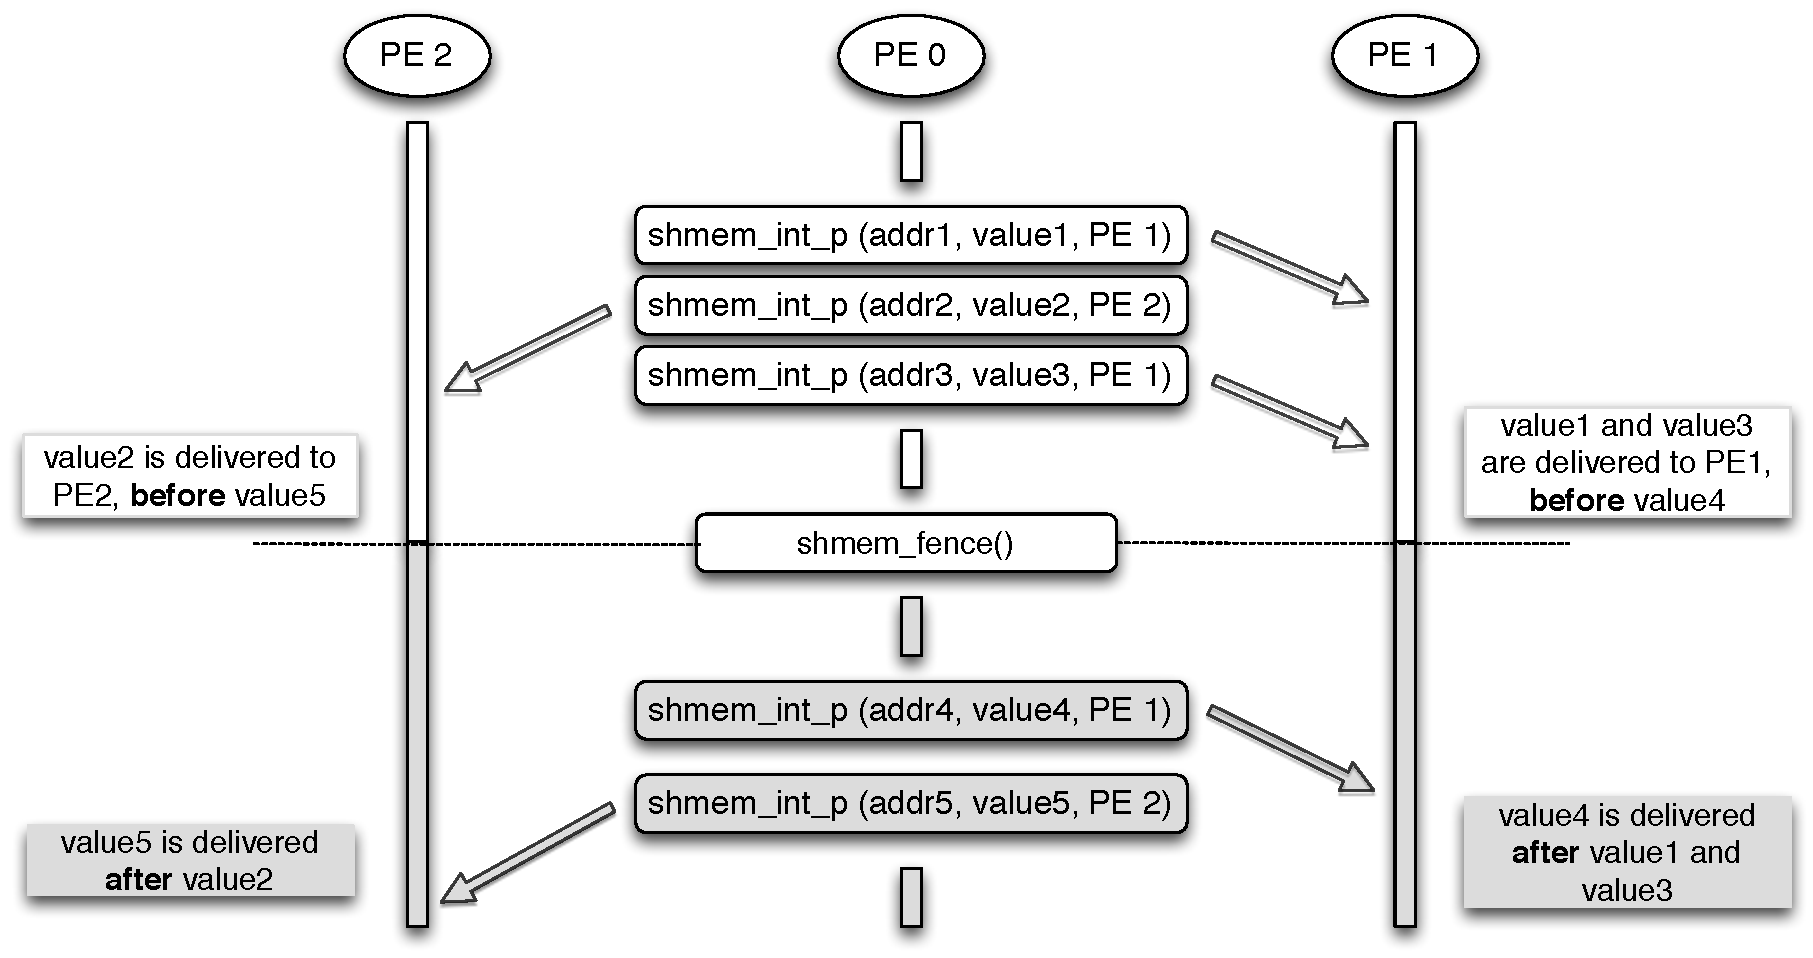
\includegraphics[width=0.7\textwidth]{diagrams/updated/fence}}
\end{tabular}

\begin{tabular}{p{0.2\textwidth} | p{0.7\textwidth}}
{}
&
All puts issued to a specific remote \ac{PE} before the fence operation by the local \ac{PE} are guaranteed to be delivered before puts issued after the fence call. This operation should be used when all remote writes by a local \ac{PE} to a specific remote \ac{PE} need to be visible %(\rcomment{Swaroop: assuming visible == delivered}) 
before any new remote write operation to the same \ac{PE}. \tabularnewline
\hline 
\end{tabular}

\begin{tabular}{p{0.2\textwidth} | p{0.7\textwidth}}
Ordering puts issued by all \ac{PE} \\
\FUNC{shmem\_quiet}
& 
\raisebox{-\totalheight}{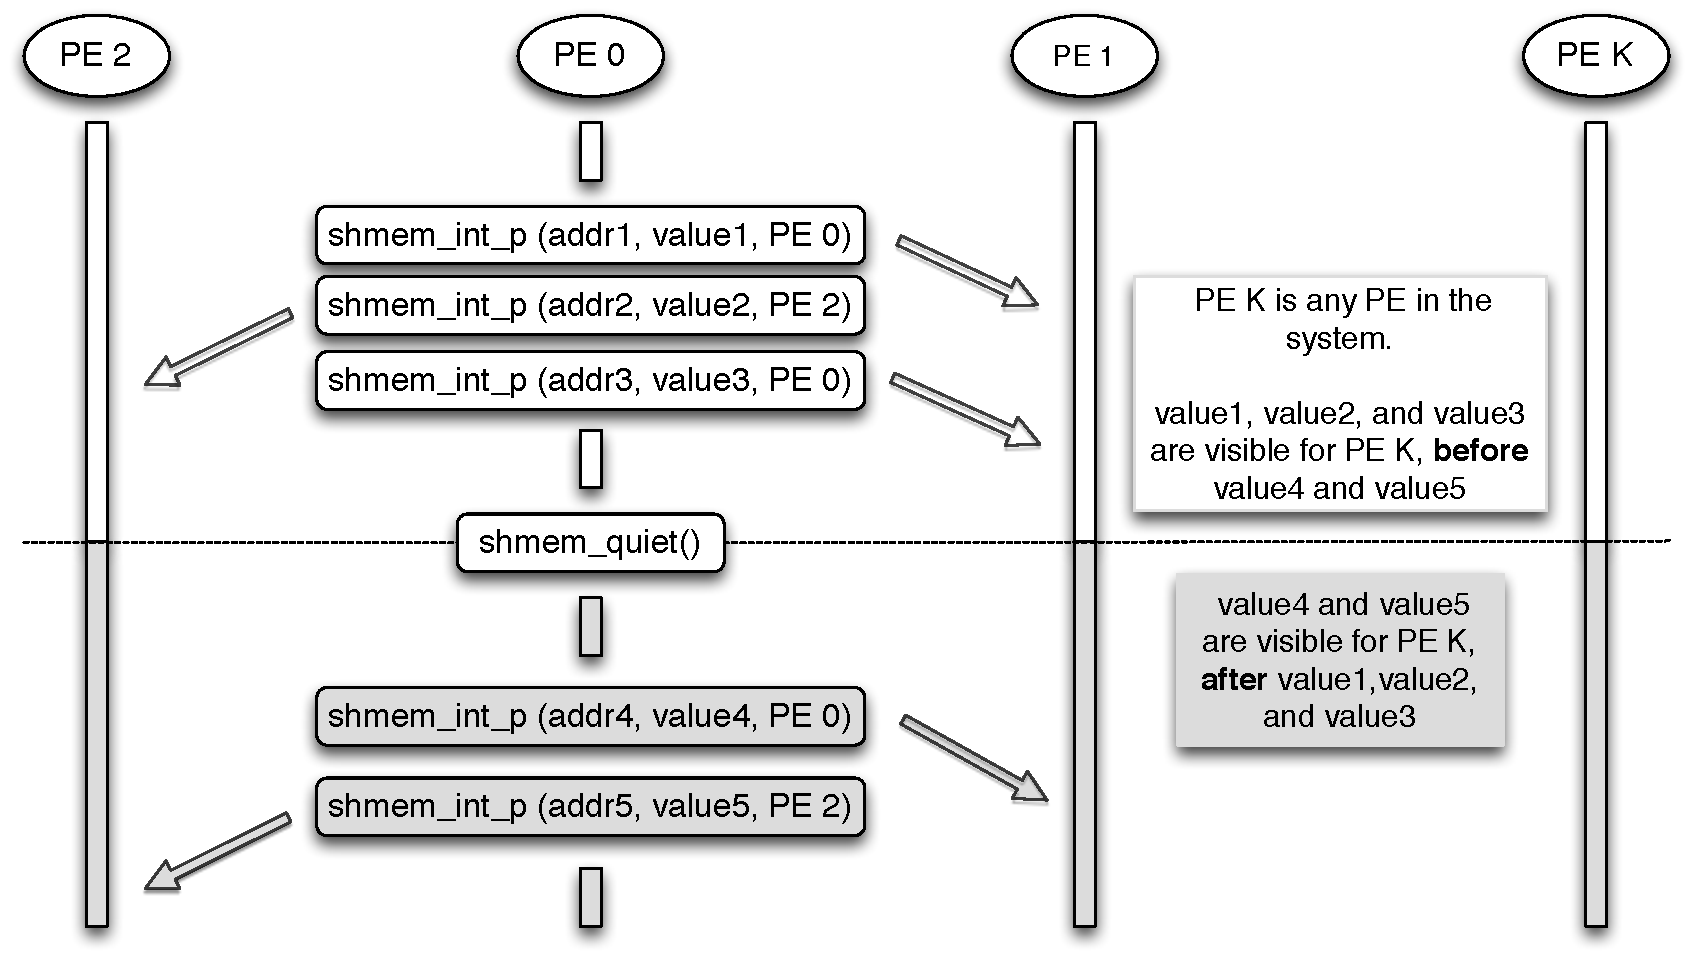
\includegraphics[width=0.7\textwidth]{diagrams/updated/quiet}} 
\end{tabular}

\begin{tabular}{p{0.2\textwidth} | p{0.7\textwidth}}
{}
&
{All puts issued by all \ac{PE}s are guaranteed to be delivered before the next local update or remote memory update via \openshmem (\rcomment{May change after SGI's input.}). This operation should be used when all remote writes by all \ac{PE}s need to be visible  to all other \ac{PE}s before any new local update or remote memory update via \openshmem library operation. } \tabularnewline
\hline 
\end{tabular}


\begin{tabular}{p{0.2\textwidth} | p{0.7\textwidth}}
Collective synchronization over an \activeset \\
\FUNC{shmem\_barrier}
&  
\raisebox{-\totalheight}{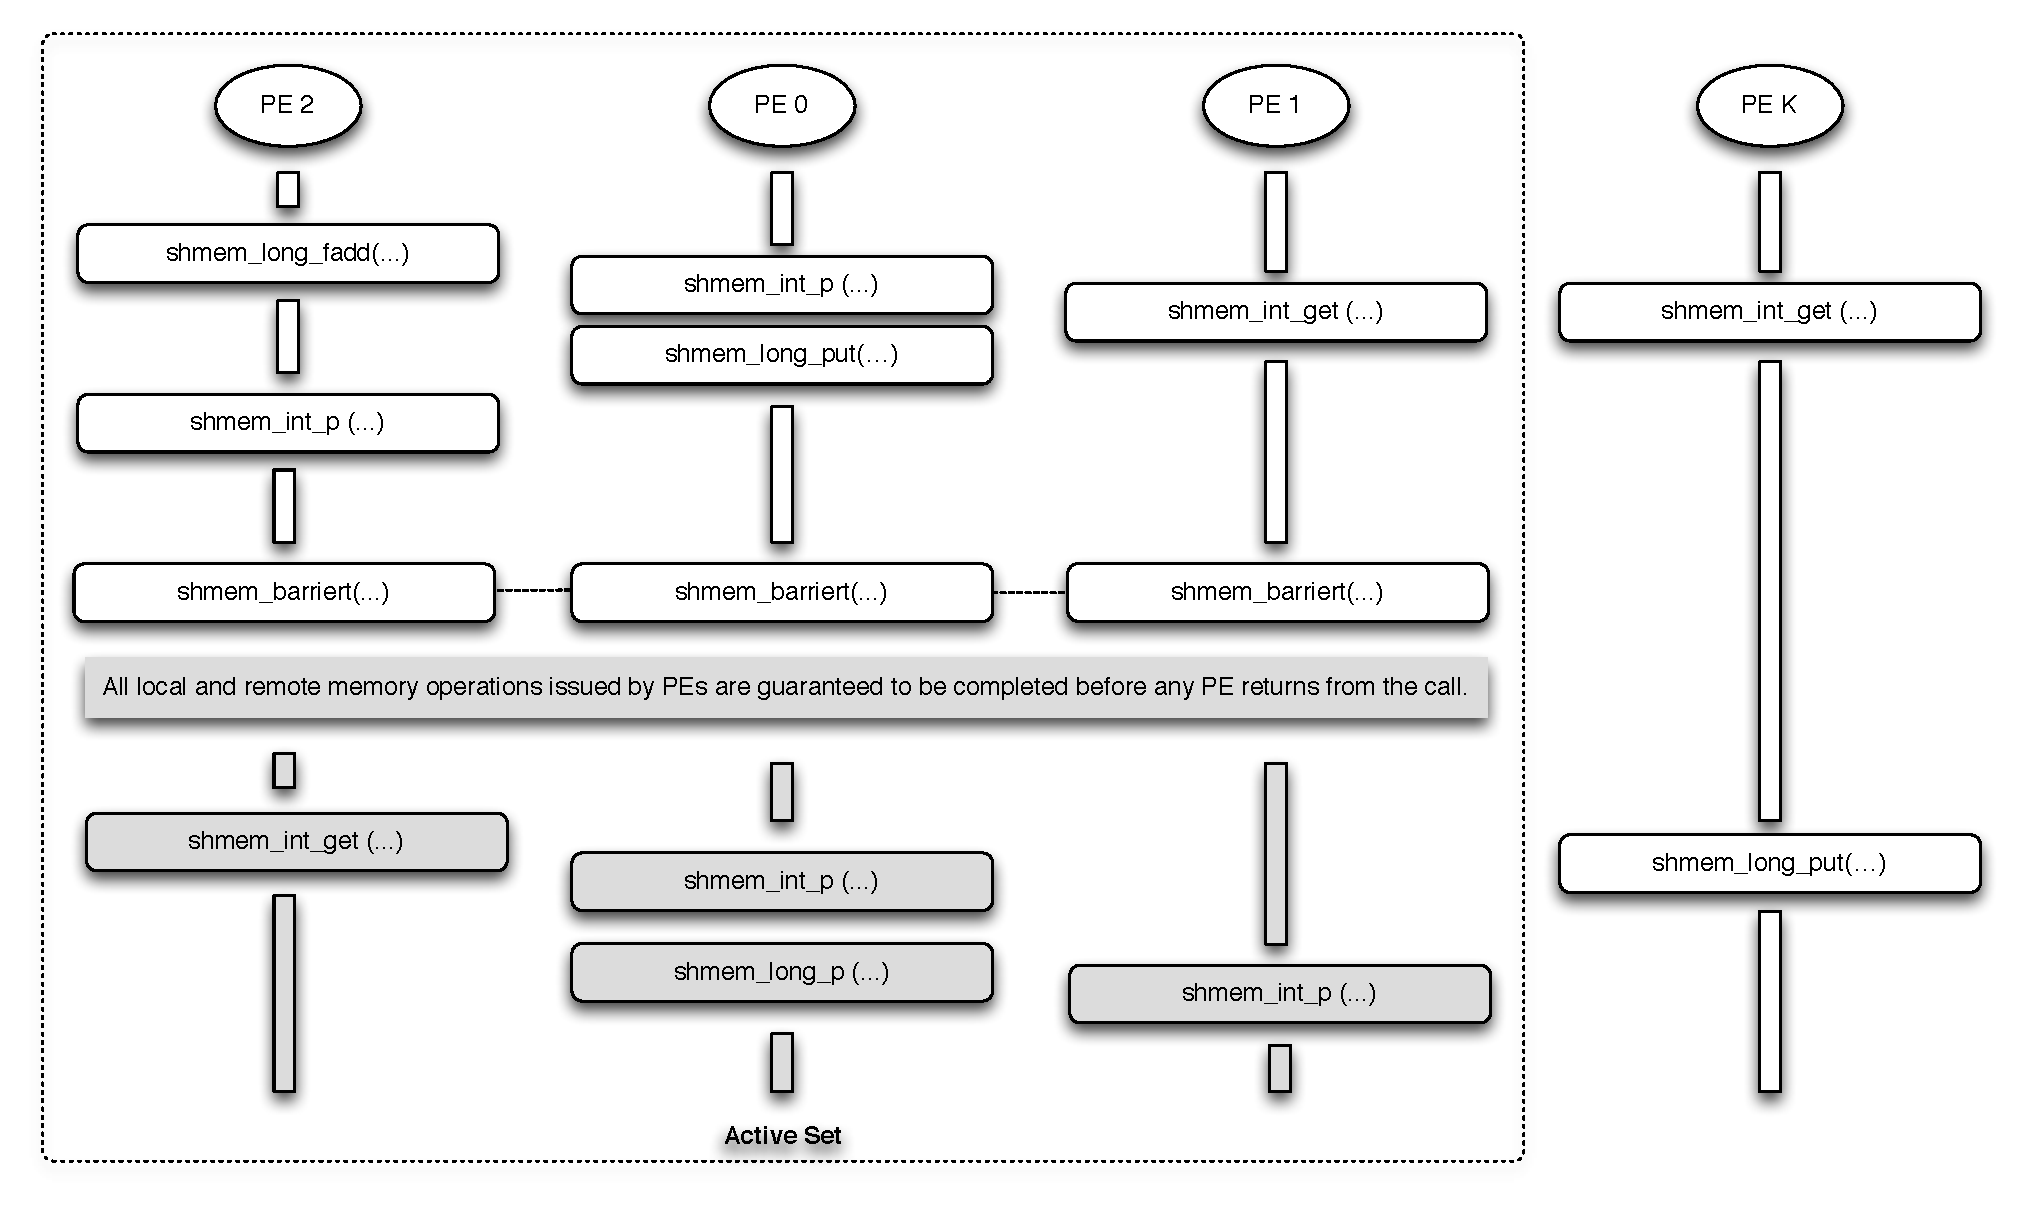
\includegraphics[width=0.7\textwidth]{diagrams/updated/barrier}} 
\end{tabular}

\begin{tabular}{p{0.2\textwidth} | p{0.7\textwidth}}
{}
&
{All local and remote memory operations issued by all \ac{PE}s within the \activeset{} are guaranteed to be completed before any \ac{PE} in the \activeset{} returns from the call. Additionally, no \ac{PE} my return from the barrier till all \ac{PE}s in the \activeset{} have called the same barrier call. This operation should be used when synchronization as well as completion of local stores and remote memory updates via \openshmem is required over a sub-set of the executing \ac{PE}s.} \tabularnewline %Figure (\ref{fig:barrier}).
\hline 
\end{tabular}

\begin{tabular}{p{0.2\textwidth} | p{0.7\textwidth}}
Collective synchronization over all \ac{PE}s \\
 \FUNC{shmem\_barrier\_all}
& 
\raisebox{-\totalheight}{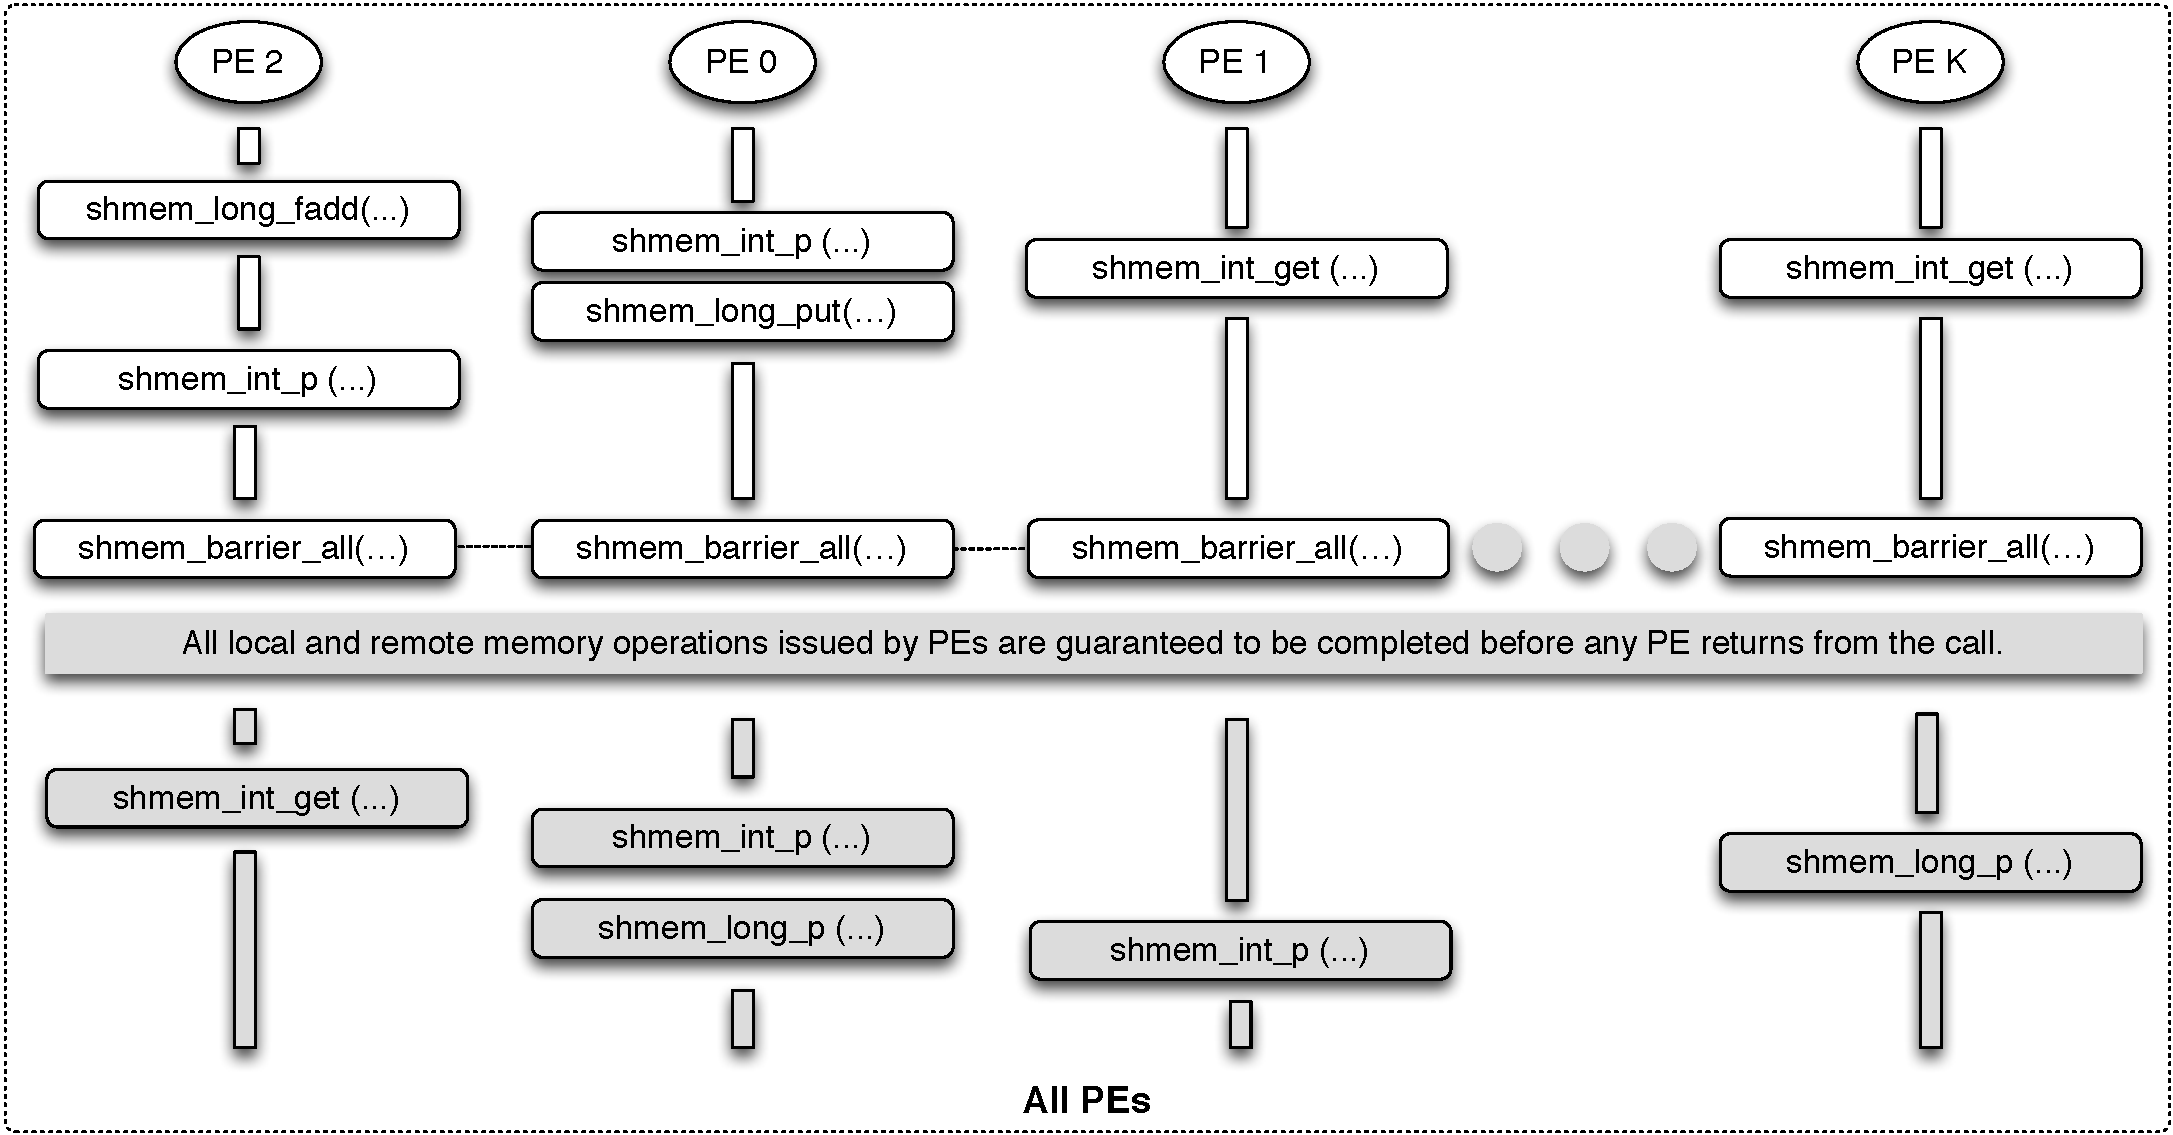
\includegraphics[width=0.7\textwidth]{diagrams/updated/barrierall}}
\end{tabular}

\begin{tabular}{p{0.2\textwidth} | p{0.7\textwidth}}
{}
&
{All local and remote memory operations issued by all \ac{PE}s are guaranteed to be completed before any \ac{PE} returns from the call. Additionally no \ac{PE} my return from the barrier until all \ac{PE}s have called the same barrier call. This operation should be used when synchronization as well as completion of local stores and remote memory updates via \openshmem is required over all \ac{PE}s. } \tabularnewline
\hline 
\end{tabular}
\clearpage
%%%%%%%%%%%%%%%%%OLD LAYOUT%%%%%%%%%%%%%%%%
%\begin{tabular}{|p{0.2\textwidth}|p{0.4\textwidth}|p{0.3\textwidth}|}
%\hline 
%\textbf{\openshmem  \ac{API}} & \centering \textbf{Working of \openshmem \ac{API}} & \textbf{Appropriate Situation}\tabularnewline
%\hline 
%\hline 
%{Point-to-point synchronization}\\
%\FUNC{shmem\_wait}, \FUNC{shmem\_wait\_until} 
%&
%\raisebox{-\totalheight}{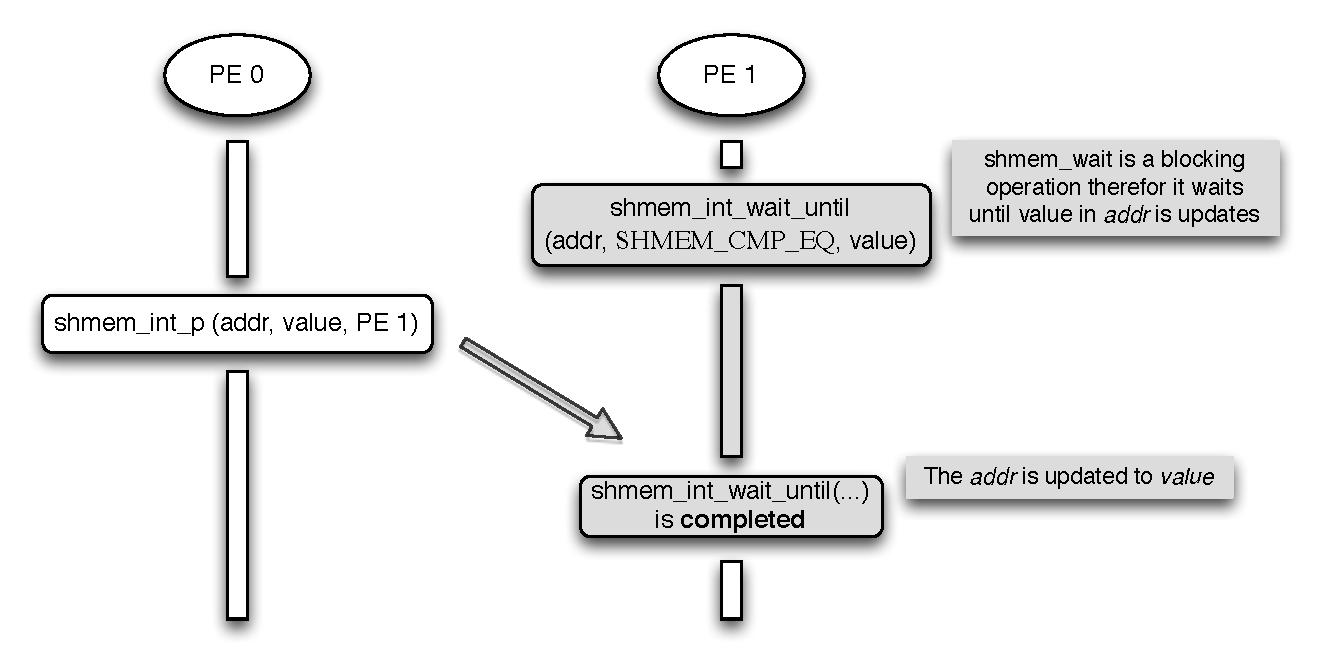
\includegraphics[width=0.39\textwidth]{diagrams/updated/wait}}
%{Waits for a symmetric variable to be updated by a remote \ac{PE}. Should be used when computation at the local \ac{PE} cannot proceed without the value that the remote \ac{PE} is to update.} \tabularnewline
%% Figure (\ref{fig:wait}).}\tabularnewline
%\hline 
%Ordering puts issued by a local \ac{PE} \\
%\FUNC{shmem\_fence} 
%& 
%\raisebox{-\totalheight}{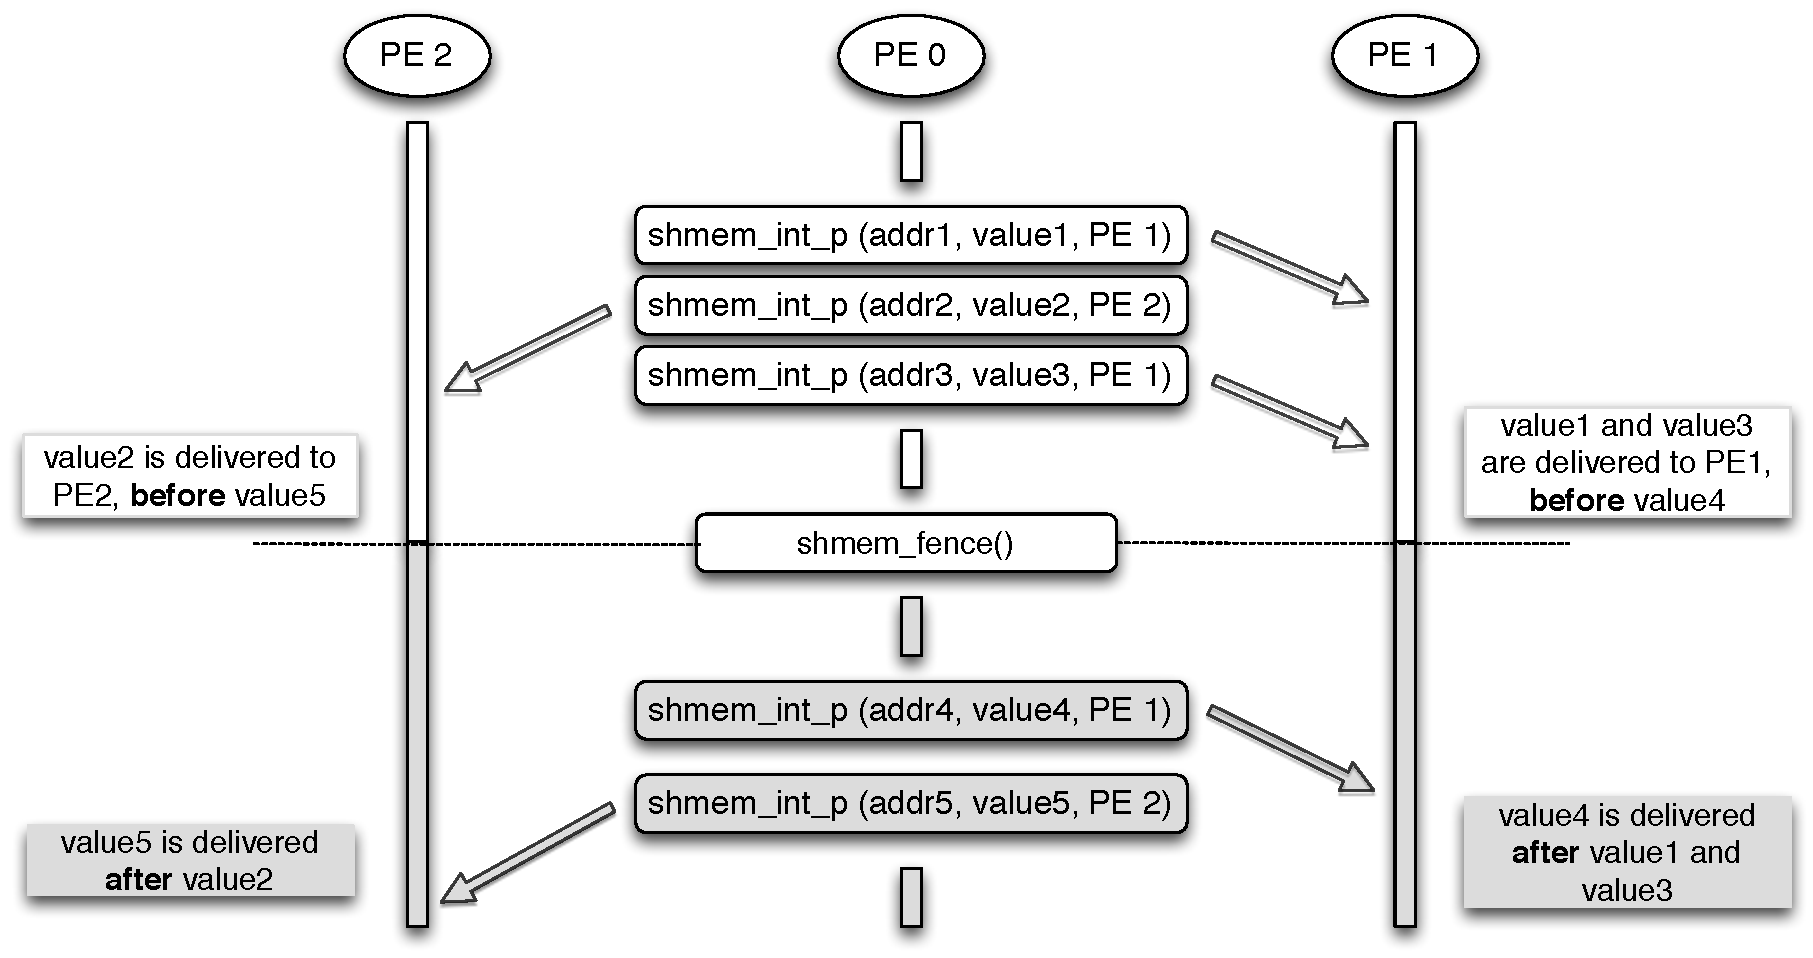
\includegraphics[width=0.39\textwidth]{diagrams/updated/fence}}
%& 
%All puts issued before the fence operation by the local \ac{PE} are guaranteed to be delivered before puts issued after the fence call to the same remote \ac{PE}. This operation should be used when all remote writes by a local \ac{PE} to a remote \ac{PE} need to be visible %(\rcomment{Swaroop: assuming visible == delivered}) 
%before any new remote write operation to the same \ac{PE}. \tabularnewline
%%Figure (\ref{fig:fence}).\tabularnewline
%\hline 
%Ordering puts issued by all \ac{PE} \\
%\FUNC{shmem\_quiet}
%& 
%\raisebox{-\totalheight}{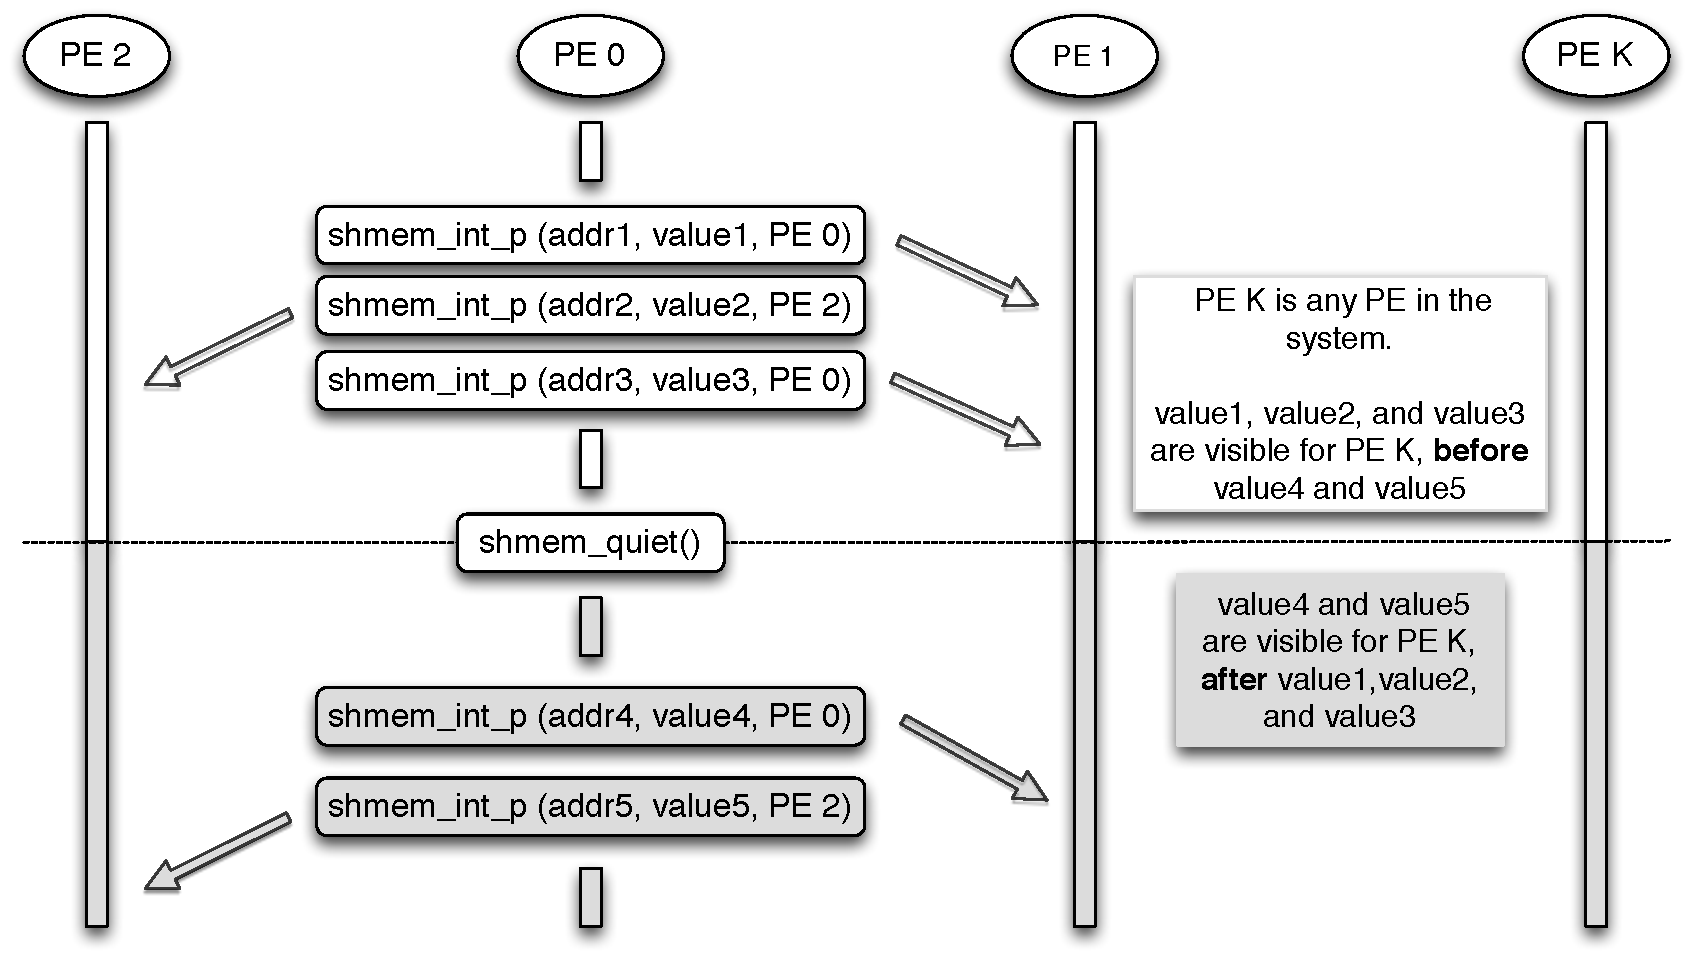
\includegraphics[width=0.39\textwidth]{diagrams/updated/quiet}} 
%& 
%{All puts issued by all \ac{PE}s are guaranteed to be delivered before the next local update or remote memory update via \openshmem (\rcomment{May change after SGI's input.}). This operation should be used when all remote writes by all \ac{PE}s need to be visible  to all other \ac{PE}s before any new local or remote memory update via \openshmem library operation. } \tabularnewline
%%Figure (\ref{fig:quiet}).} \tabularnewline
%\hline 
%\end{tabular}
%\clearpage
%\begin{tabular}{|p{0.2\textwidth}|p{0.4\textwidth}|p{0.3\textwidth}|}
%\hline 
%Collective synchronization over an \activeset \\
%\FUNC{shmem\_barrier}
%&  
%\raisebox{-\totalheight}{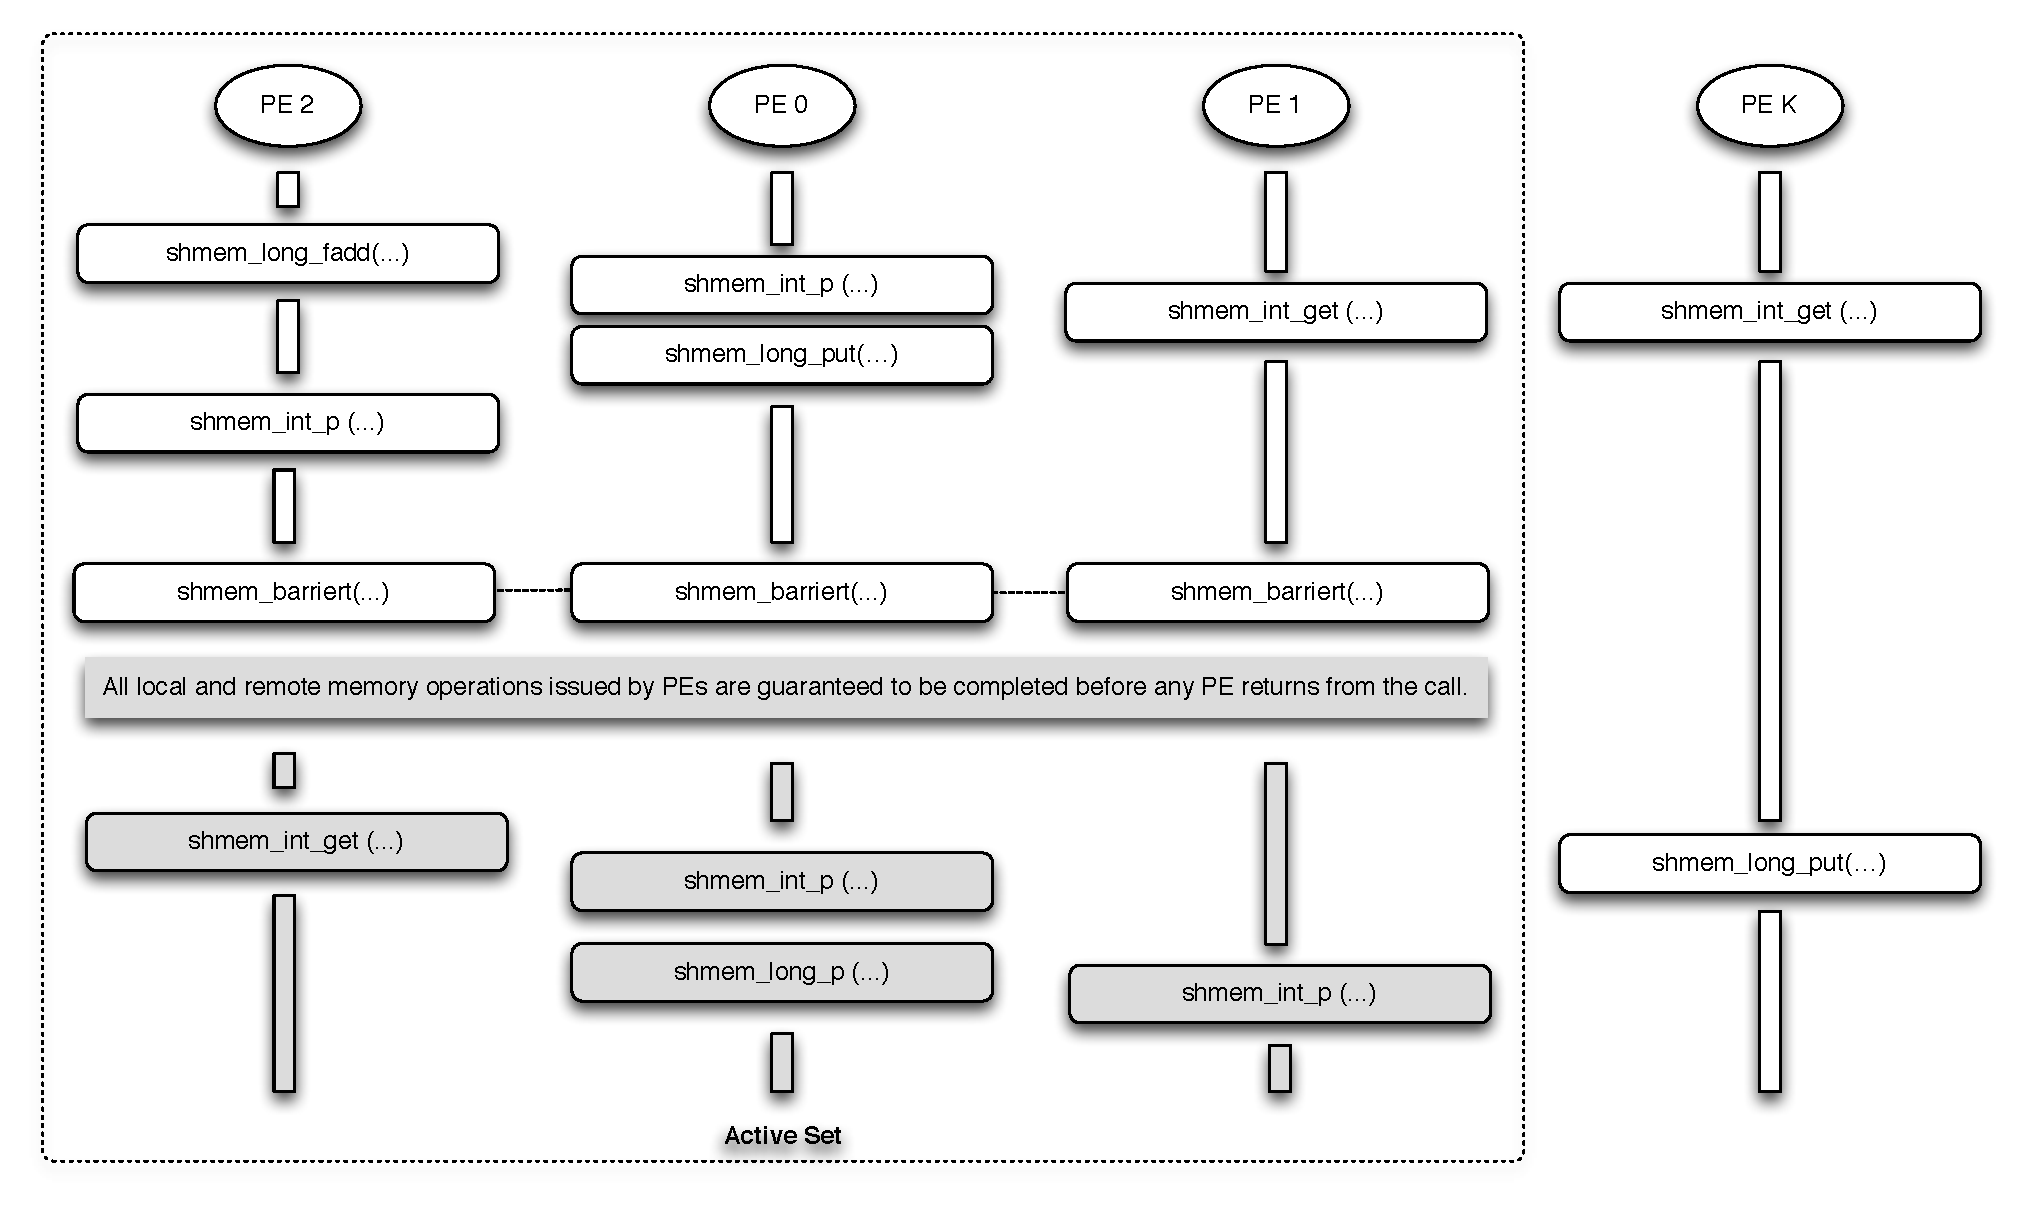
\includegraphics[width=0.39\textwidth]{diagrams/updated/barrier}} 
%& 
%{All local and remote memory operations issued by all \ac{PE}s within the \activeset{} are guaranteed to be completed before any \ac{PE} in the \activeset{} returns from the call. Additionally no \ac{PE} my return from the barrier till all \ac{PE}s in the \activeset{} have called the same barrier call. This operation should be used when synchronization as well as completion of local stores and remote memory updates via \openshmem is required over a sub-set of the executing \ac{PE}s.} \tabularnewline %Figure (\ref{fig:barrier}).
%\hline 
%Collective synchronization over all \ac{PE}s \\
% \FUNC{shmem\_barrier\_all}
%& 
%\raisebox{-\totalheight}{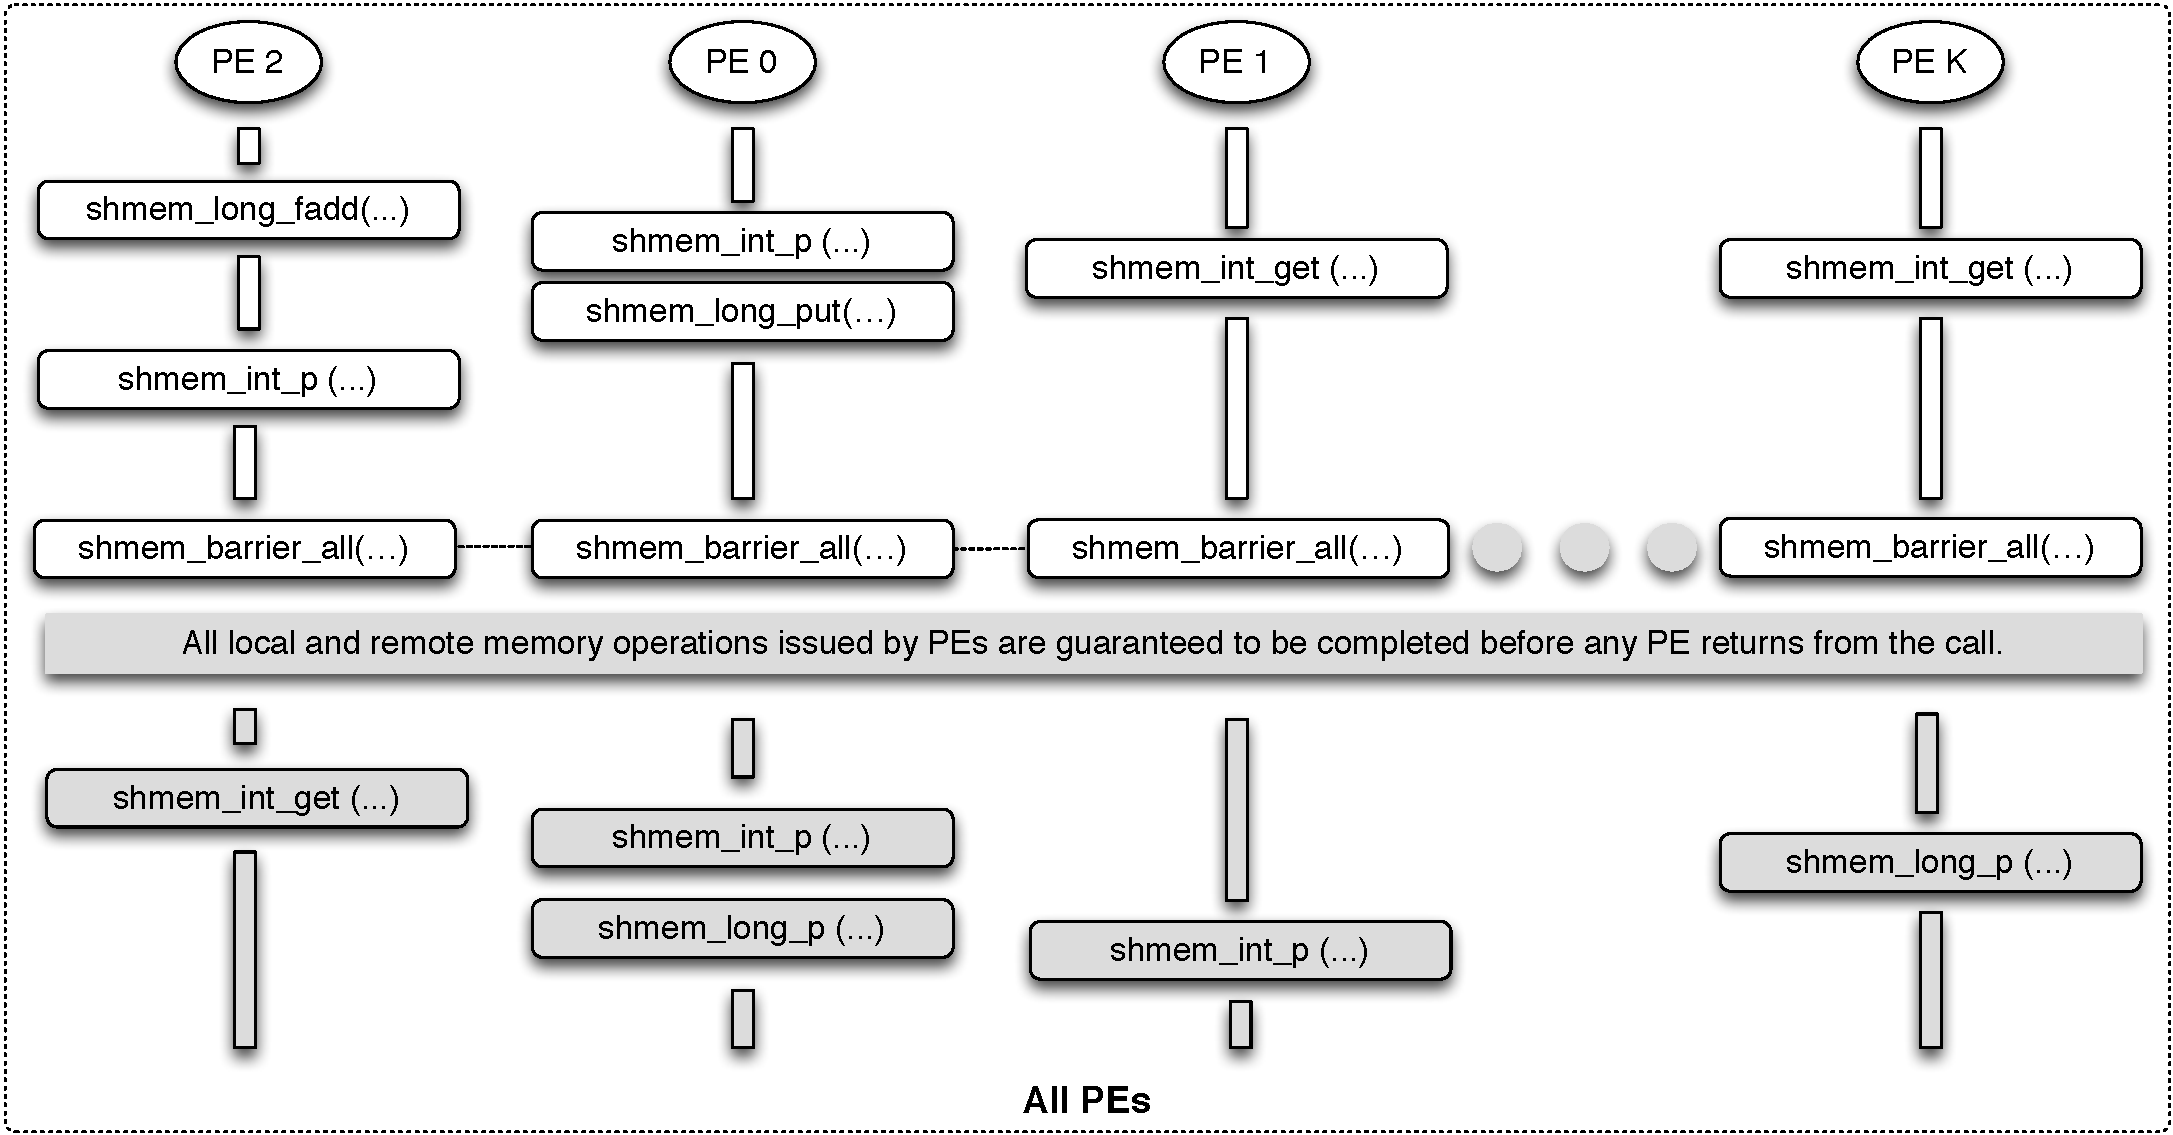
\includegraphics[width=0.39\textwidth]{diagrams/updated/barrierall}}
%& 
%{All local and remote memory operations issued by all \ac{PE}s are guaranteed to be completed before any \ac{PE} returns from the call. Additionally no \ac{PE} my return from the barrier until all \ac{PE}s have called the same barrier call. This operation should be used when synchronization as well as completion of local stores and remote memory updates via \openshmem is required over all \ac{PE}s. } \tabularnewline%Figure (\ref{fig:barrierall}).
%
%\hline 
%\end{tabular}


%\begin{figure}
%%        \centering
%        \begin{subfigure}{0.5\textwidth}
%                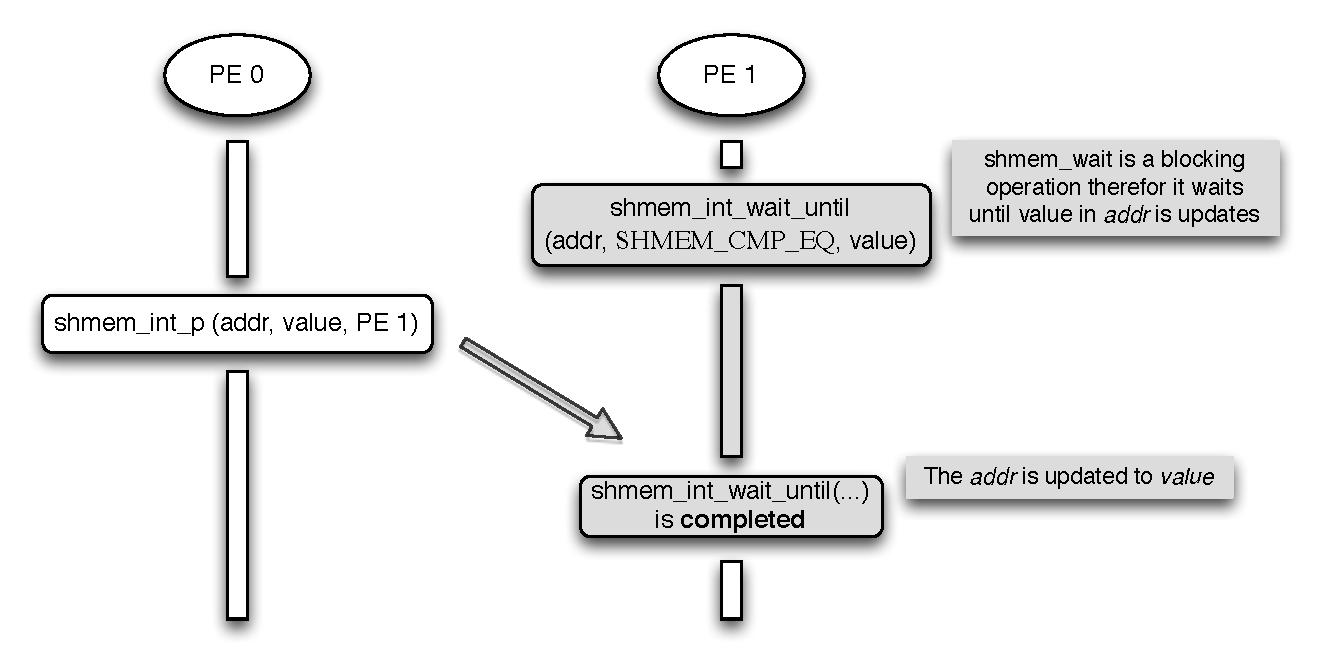
\includegraphics[width=\textwidth]{diagrams/updated/wait}
%                \caption{\FUNC{shmem\_wait}}
%                \label{fig:wait}
%        \end{subfigure}
%        \begin{subfigure}{0.49\textwidth}
%                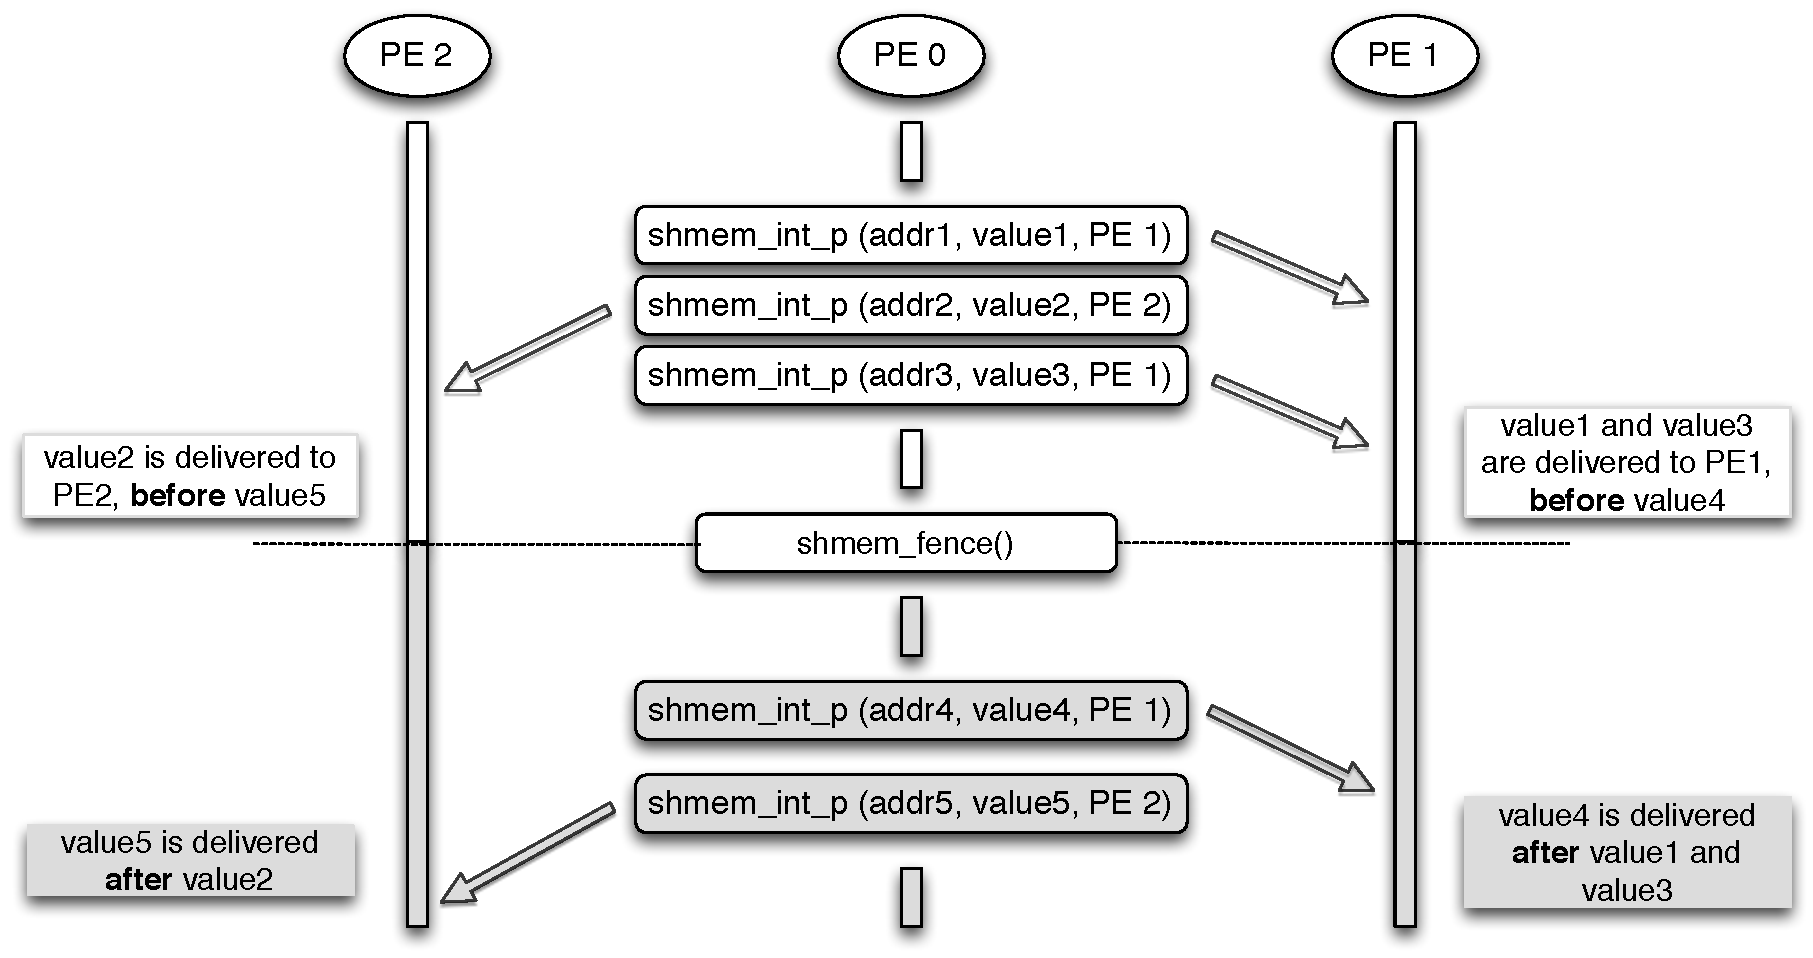
\includegraphics[width=\textwidth]{diagrams/updated/fence}
%                \caption{\FUNC{shmem\_fence}}
%                \label{fig:fence}
%        \end{subfigure}
%        \begin{subfigure}{0.48\textwidth}
%                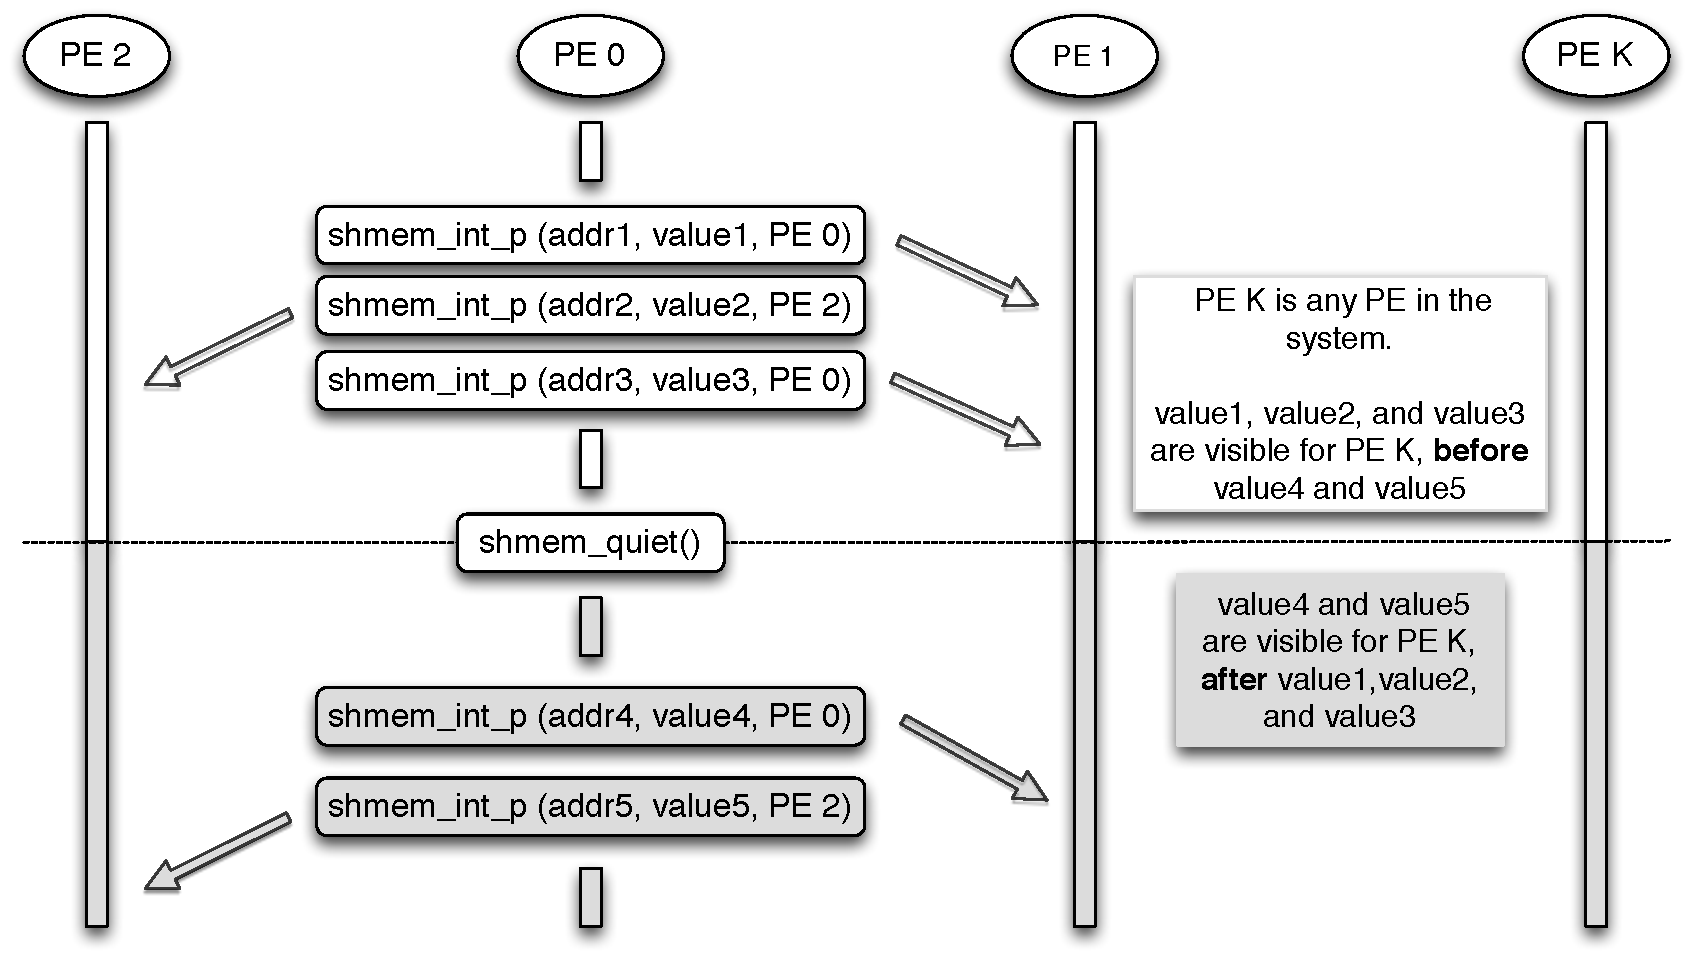
\includegraphics[width=\textwidth]{diagrams/updated/quiet}
%                \caption{\FUNC{shmem\_quiet}}
%                \label{fig:quiet}
%        \end{subfigure}
%	    \begin{subfigure}{0.48\textwidth}
%		        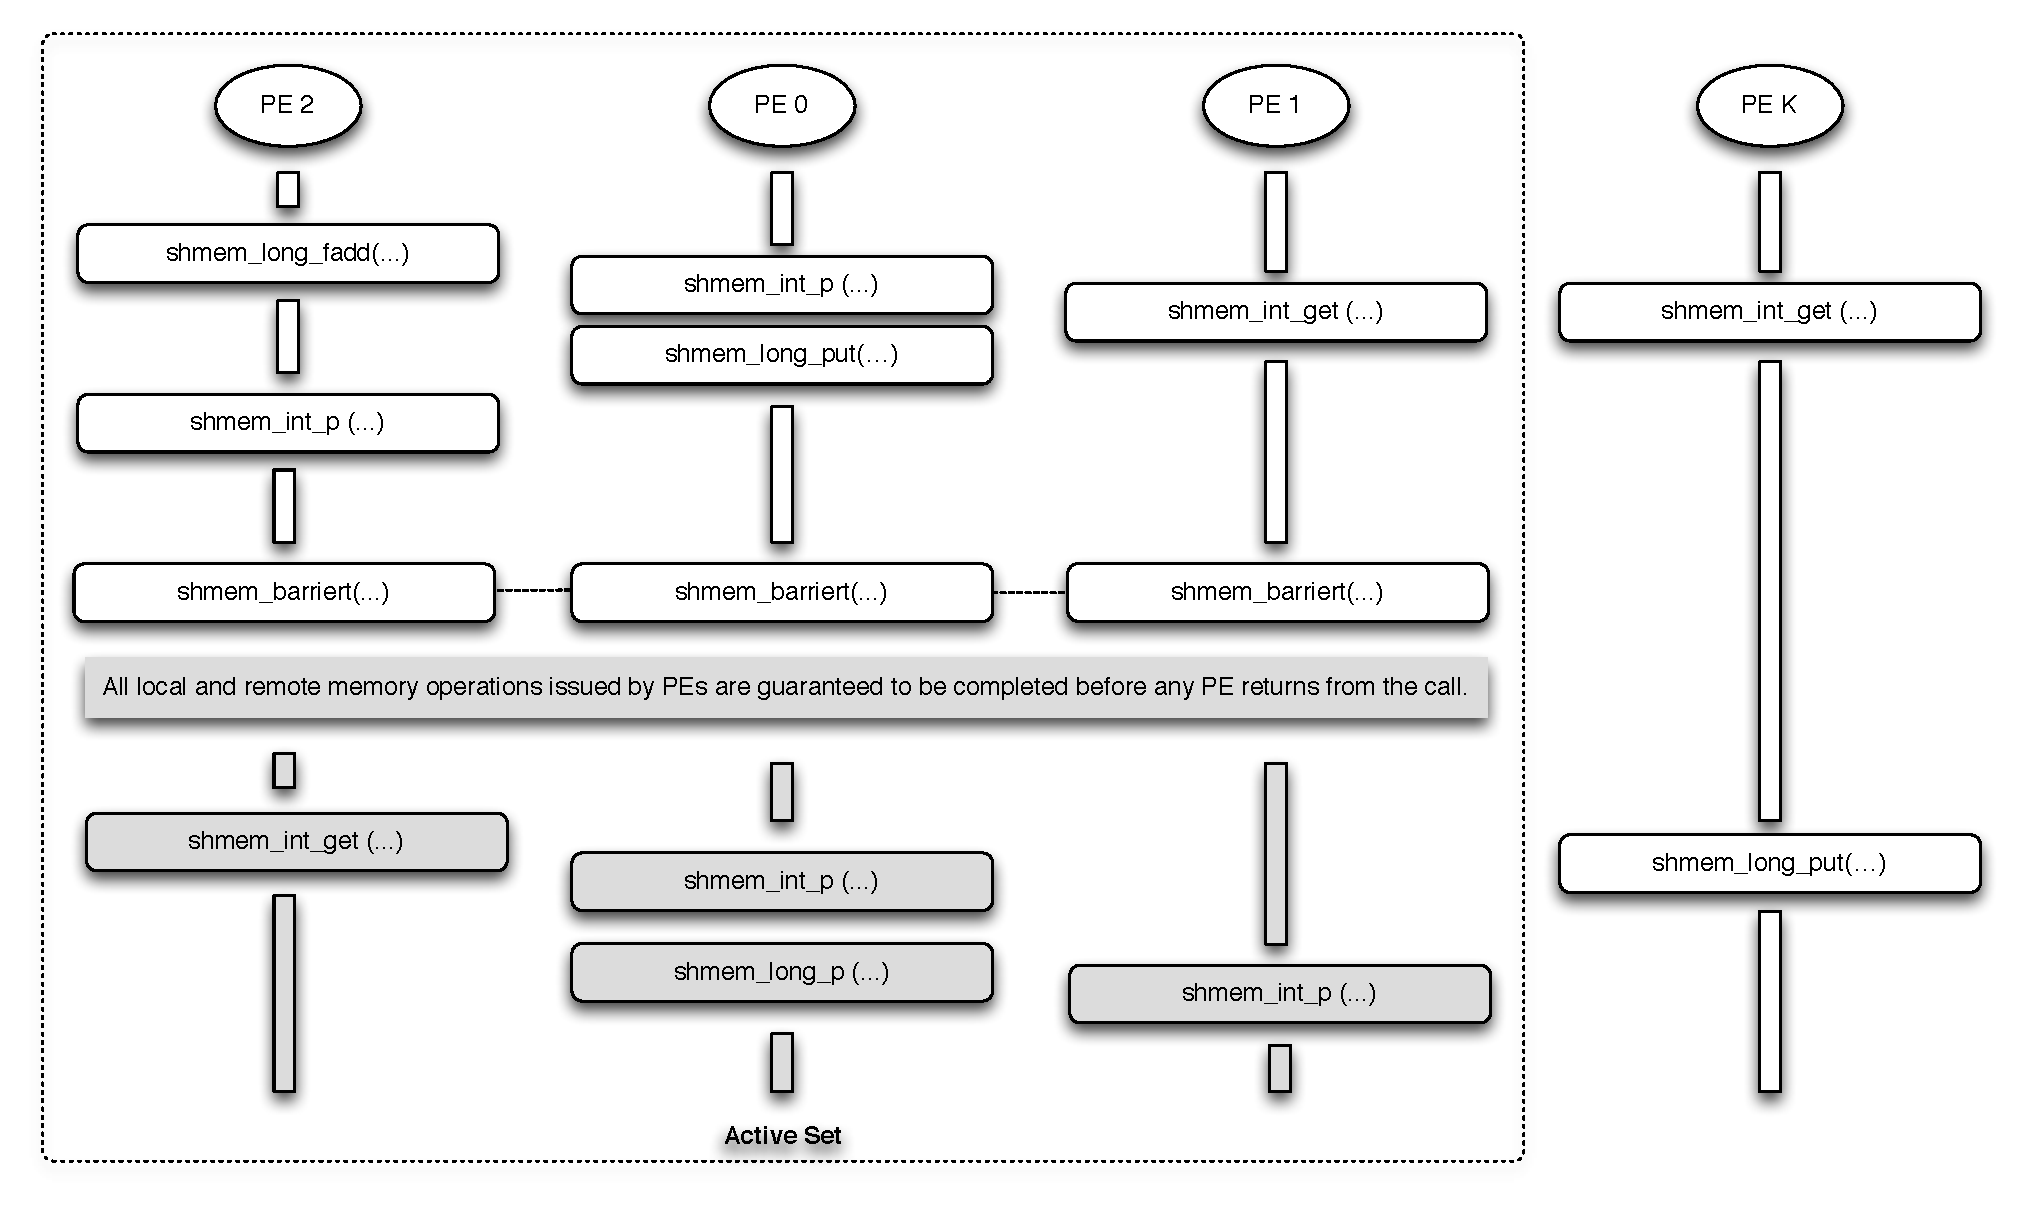
\includegraphics[width=\textwidth]{diagrams/updated/barrier}
%		        \caption{\FUNC{shmem\_barrier}}
%		\label{fig:barrier}
%	    \end{subfigure}
%        \centering
%	    \begin{subfigure}{0.48\textwidth}
%		        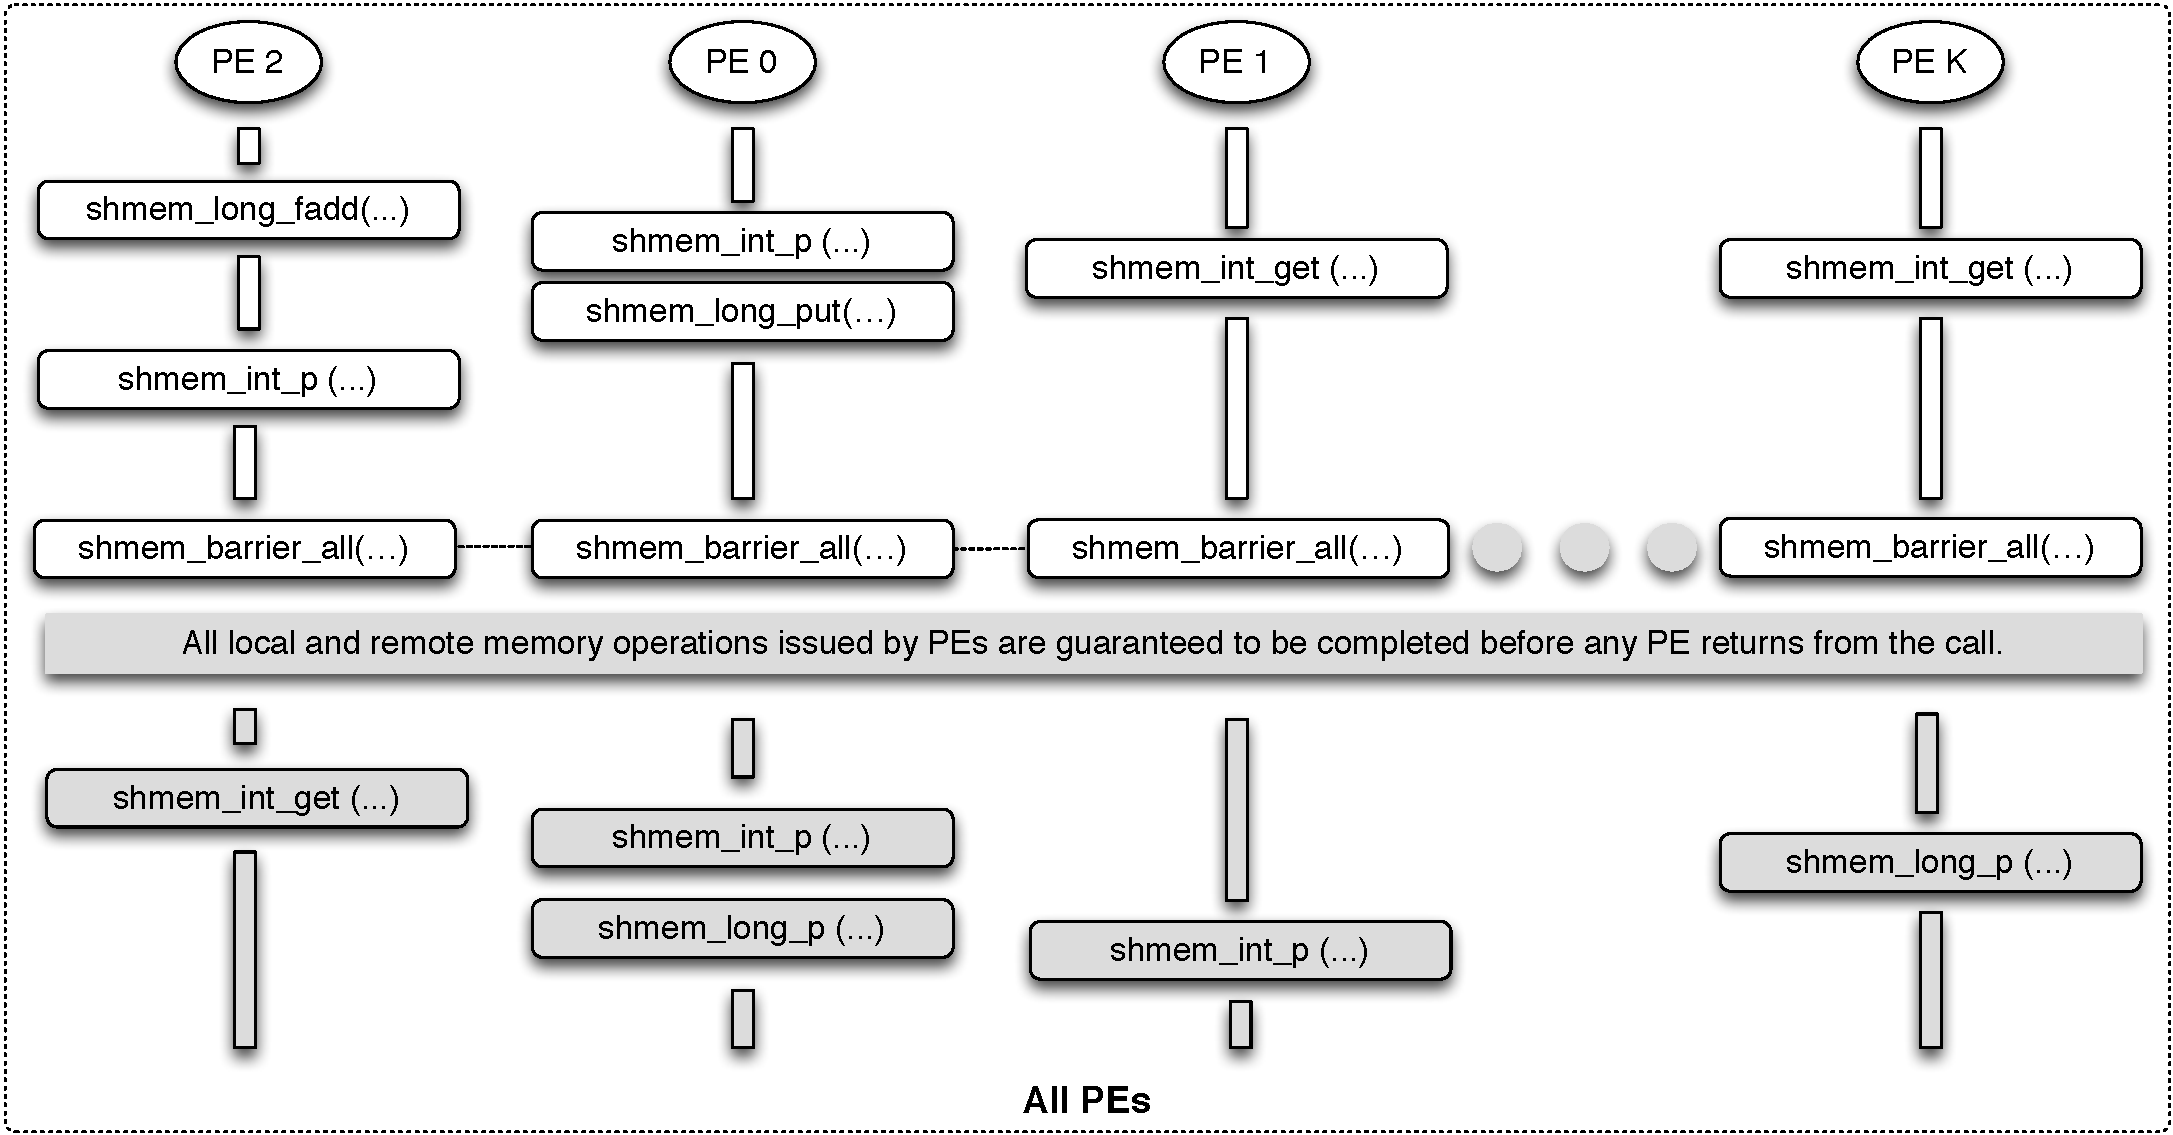
\includegraphics[width=\textwidth]{diagrams/updated/barrierall}
%		        \caption{\FUNC{shmem\_barrierall}}
%		\label{fig:barrierall}
%	    \end{subfigure}
%        \caption{\openshmem{} synchronization operations}\label{fig:animals}
%\end{figure}
